\documentclass[12pt]{article}
\usepackage[utf8]{inputenc}
\usepackage[russian]{babel}
\usepackage{graphicx}
\usepackage{array}
\usepackage[a4paper, left=1cm, right=1cm, top=1.27cm, bottom=1.27cm]{geometry}
\usepackage{setspace}
\usepackage{tabularx}
\usepackage{makecell}
\usepackage{longtable}
\usepackage{multirow}
\usepackage{caption}
\onehalfspacing


\begin{document}


\begin{table}[h]
    \centering
    \renewcommand{\arraystretch}{1.5} % Увеличиваем межстрочный интервал
    \begin{tabular}{|m{11cm}|m{6cm}|} % Первая колонка шире, вторая для лого
        \hline
        \begin{center}
            \textbf{Университет ITMO}\\
            \textbf{Физико-технический мегафакультет}\\
            \textbf{Физический факультет}
        \end{center} 
        & 
        \begin{center}
            
\includegraphics[height=1.3cm]{logo.jpg}
        \end{center} \\
        \hline
    \end{tabular}
\end{table}

\noindent\makebox[\linewidth]{\rule{\textwidth}{2pt}}

\vspace{10pt}

\begin{table}[h]
    \centering
    \renewcommand{\arraystretch}{1.7}
    \begin{tabular}{|p{4cm}p{4cm}|p{8cm}|}
        \hline
        Группа N3150 & & К работе допущен \underline{\hspace{4cm}} \\
        \hline
        Студенты & \hfill \multirow[0pt]{3}{*}{\makecell[c]{Пахомов В.Ю \\ Фармахини Ф.Р. \\ Петров Д.О}}  & Работа выполнена \underline{\hspace{4cm}} \\
        & & \\
        & & \\
        \hline
        \multicolumn{2}{|c|}{Преподаватель \underline{\hspace{5cm}}}  & Отчет принят \underline{\hspace{5cm}} \\
        \hline
    \end{tabular}
\end{table}

\begin{center}
    \fontsize{20pt}{21.5pt} \selectfont
    \textbf{Рабочий протокол и отчет по}\\
    \textbf{лабораторной работе № 1.03}
\end{center}

\noindent\makebox[\linewidth]{\rule{\textwidth}{1pt}}
\noindent\makebox[\linewidth]{\rule{\textwidth}{1pt}}

\begin{flushleft}
    1. Цель работы.\\
    \hspace{0.63cm}1) Исследование упругого и неупругого центрального соударения тел на примере тележек, движущихся с малым трением. \\
    \hspace{0.63cm}2) Исследование зависимости ускорения тележки от приложенной силы и массы тележки.
\end{flushleft}

\begin{flushleft}
    2. Задачи, решаемые при выполнении работы.\\
    \hspace{0.63cm}1) Измерение скоростей тележек до и после соударения. \\
    \hspace{0.63cm}2) Измерение скорости тележки при ее разгоне под действием постоянной силы. \\
    \hspace{0.63cm}3) Исследование потерь импульса и механической энергии при упругом и неупругом соударении двух тележек. \\
    \hspace{0.63cm}4) Исследование зависимости ускорения тележки от приложенной силы и массы тележки. Проверка второго закона Ньютона. \\
\end{flushleft}

\begin{flushleft}
    3. Объект исследования. \\
    Две тележки, движущиеся по горизонтальному рельсу с малым трением. Изучается
    их взаимодействие при центральном упругом и неупругом соударениях, а также
    движение тележки под действием внешней силы (гирьки, подвешенной через блок). \\
\end{flushleft}

\begin{flushleft}
    4. Метод экспериментального исследования. \\
    Исследование соударений и проверка второго закона Ньютона. \\
\end{flushleft}

\begin{flushleft}
    5. Рабочие формулы и исходные данные. \\
    $ p_{10x} = m_1 v_{10x}, $ \\
    $ p_{1x} = m_1 v_{1x}, $ \\
    $ p_{2x} = m_2 v_{2x} $ \\
    $ \delta_p = \frac{\Delta p_x}{p_{10x}} = \left( \frac{p_{1x} + p_{2x}}{p_{10x}} \right) - 1 $ \\
    $ \delta_W = \frac{\Delta W_k}{W_{k0}} = \frac{m_1 v_{1x}^2 + m_2 v_{2x}^2}{m_1 v_{10x}^2} - 1 $ \\ 
    $ \bar{\delta}_p = \frac{1}{N} \sum_{i=1}^N \delta_{pi}, $ \\
    $ \bar{\delta}_W = \frac{1}{N} \sum_{i=1}^N \delta_{Wi} $ \\
    $ \Delta \bar{\delta}_p = t_{\alpha_{dov},N} \cdot \sqrt{\frac{\sum_{i=1}^N (\delta_{pi} - \bar{\delta}_p)^2}{N(N - 1)}}, $ \\
    $ \Delta \bar{\delta}_W = t_{\alpha_{dov},N} \cdot \sqrt{\frac{\sum_{i=1}^N (\delta_{Wi} - \bar{\delta}_W)^2}{N(N - 1)}} $ \\
    $ \delta_W^{(E)} = \frac{\Delta W_k}{W_{k0}} = \left( \frac{(m_1 + m_2) v_0^2}{m_1 v_{10}^2} \right) - 1 $ \\
    $ \delta_W^{(T)} = \frac{-W_{pot}}{\frac{m_1 v_{10}^2}{2}} = -\frac{m_2}{m_1 + m_2} $ \\
\end{flushleft}

\begin{flushleft}
    6. Измерительные приборы. \\
    \begin{table}[h]
        \centering
        \renewcommand{\arraystretch}{1.5}
        {\itshape
        \begin{tabular}{|c|c|c|c|c|}
            \hline
            № п/п & Наименование & Тип прибора & Используемый диапазон & Погрешность прибора\\
            \hline
            1 & Весы & Электронный & 250 г & ±0.01 г \\
            \hline
            2 & Линейка на рельсе & Вычислительный & 1.3 м & ±0.5 см \\
            \hline
            3 & Оптические ворота & Электронный & - & - \\
            \hline
            4 & ПКЦ-3 & Электронный & 0-9.99 м/c & ±0.01 м/c \\
            \hline
        \end{tabular}
        }
    \end{table}
\end{flushleft}


\newpage


\begin{flushleft}
    7. Схема установки. \\
    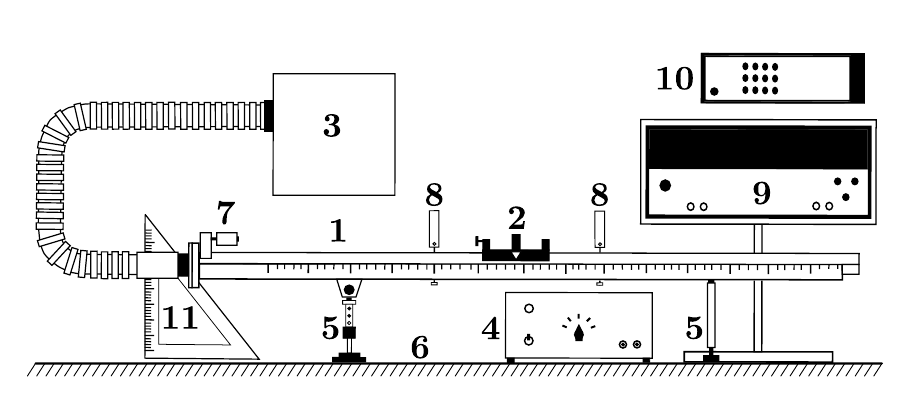
\includegraphics[height=8cm]{shema.png} \\
    \hspace{0.63cm}1) Рельс с сантиметровой шкалой на лицевой стороне \\
    \hspace{0.63cm}2) Сталкивающиеся тележки \\ 
    \hspace{0.63cm}3) Воздушный насос \\
    \hspace{0.63cm}4) Источник питания насоса ВС 4-12 \\
    \hspace{0.63cm}5) Опоры рельса \\
    \hspace{0.63cm}6) Опорная плоскость (поверхность стола) \\
    \hspace{0.63cm}7) Фиксирующий электромагнит \\
    \hspace{0.63cm}8) Оптические ворота \\
    \hspace{0.63cm}9) Цифровой измерительный прибор ПКЦ-3 \\
    \hspace{0.63cm}10) Пульт дистанционного управления прибором ПКЦ-3 \\
\end{flushleft}


\begin{flushleft}
    8. Результаты прямых измерений и их обработки. \\

    \begin{table}[h]
        \centering
        \renewcommand{\arraystretch}{1.3}
        \setlength{\tabcolsep}{8pt}
        \captionsetup{justification=centering, font=bf}
        \caption{Таблица 1.1}
        \begin{tabular}{|c|c|c|c|c|c|}
            \hline
            № опыта & $m_1$, г & $m_2$, г & $v_{10}$, м/с & $v_{1x}$, м/с & $ v_{2x} $ \\
            \hline
            1 & 51.09 & 49.84 & 0.52 & 0.07 & 0.49 \\
            \cline{1-1}
            \cline{4-6}
            2 &       &     & 0.51 & 0.06 & 0.48 \\
            \cline{1-1}
            \cline{4-6}
            3 &       &     & 0.50 & 0.06 & 0.47 \\
            \cline{1-1}
            \cline{4-6}
            4 &       &     & 0.52 & 0.07 & 0.48 \\
            \cline{1-1}
            \cline{4-6}
            5 &       &     & 0.51 & 0.06 & 0.49 \\
            \hline
        \end{tabular}
    \end{table}

    \newpage


    \begin{table}[h]
        \centering
        \renewcommand{\arraystretch}{1.3}
        \setlength{\tabcolsep}{8pt}
        \captionsetup{justification=centering, font=bf}
        \caption{Таблица 1.2}
        \begin{tabular}{|c|c|c|c|c|c|}
            \hline
            № опыта & $m_1$, г & $m_2$, г & $v_{10}$, м/с & $v_{1x}$, м/с & $ v_{2x} $ \\
            \hline
            1 & 51.09 & 100.64 & 0.56 & -0.12 & 0.29 \\
            \cline{1-1}
            \cline{4-6}
            2 &       &     & 0.55 & -0.19 & 0.31 \\
            \cline{1-1}
            \cline{4-6}
            3 &       &     & 0.56 & -0.12 & 0.31 \\
            \cline{1-1}
            \cline{4-6}
            4 &       &     & 0.56 & -0.17 & 0.40 \\
            \cline{1-1}
            \cline{4-6}
            5 &       &     & 0.46 & -0.13 & 0.33 \\
            \hline
        \end{tabular}
    \end{table}

    \begin{table}[h]
        \centering
        \renewcommand{\arraystretch}{1.3}
        \setlength{\tabcolsep}{8pt}
        \captionsetup{justification=centering, font=bf}
        \caption{Таблица 2.1}
        \begin{tabular}{|c|c|c|c|c|}
            \hline
            № опыта & $m_1$, г & $m_2$, г & $v_{10}$, м/с & $v$, м/с \\
            \hline
            1 & 54.29 & 52.22 & 0.61 & 0.52 \\
            \cline{1-1}
            \cline{4-5}
            2 &       &     & 0.59 & 0.51 \\
            \cline{1-1}
            \cline{4-5}
            3 &       &     & 0.62 & 0.56 \\
            \cline{1-1}
            \cline{4-5}
            4 &       &     & 0.62 & 0.54 \\
            \cline{1-1}
            \cline{4-5}
            5 &       &     & 0.6 & 0.55 \\
            \hline
        \end{tabular}
    \end{table}

    \begin{table}[h]
        \centering
        \renewcommand{\arraystretch}{1.3}
        \setlength{\tabcolsep}{8pt}
        \captionsetup{justification=centering, font=bf}
        \caption{Таблица 2.2}
        \begin{tabular}{|c|c|c|c|c|}
            \hline
            № опыта & $m_1$, г & $m_2$, г & $v_{10}$, м/с & $v$, м/с \\
            \hline
            1 & 54.30 & 103 & 0.48 & 0.15 \\
            \cline{1-1}
            \cline{4-5}
            2 &       &     & 0.49 & 0.14 \\
            \cline{1-1}
            \cline{4-5}
            3 &       &     & 0.50 & 0.15 \\
            \cline{1-1}
            \cline{4-5}
            4 &       &     & 0.48 & 0.14 \\
            \cline{1-1}
            \cline{4-5}
            5 &       &     & 0.47 & 0.13 \\
            \hline
        \end{tabular}
    \end{table}

    \newpage

    \begin{table}[h]
        \centering
        \renewcommand{\arraystretch}{1.3}
        \setlength{\tabcolsep}{8pt}
        \captionsetup{justification=centering, font=bf}
        \caption{Таблица 3.1. Разгоняемое тело – тележка 1. $M_1 = 48{,}26$}
        \begin{tabular}{|c|l|c|c|c|}
            \hline
            № опыта & Состав гирьки & $m$, г & $v_1$, м/с & $v_2$, м/с \\
            \hline
            1 & подвеска & 1.90 & 0.22 & 0.53 \\
            \hline
            2 & подвеска + одна шайба & 2.40 & 0.26 & 0.61 \\
            \hline
            3 & подвеска + две шайбы & 3.32 & 0.33 & 0.76 \\
            \hline
            4 & подвеска + три шайбы & 4.23 & 0.37 & 0.92 \\
            \hline
            5 & подвеска + четыре шайбы & 5.03 & 0.41 & 0.99 \\
            \hline
            6 & подвеска + пять шайб & 5.97 & 0.49 & 1.12 \\
            \hline
            7 & подвеска + шесть шайб & 6.52 & 0.51 & 1.18 \\
            \hline
        \end{tabular}
    \end{table}
    
    \begin{table}[h]
        \centering
        \renewcommand{\arraystretch}{1.3}
        \setlength{\tabcolsep}{8pt}
        \captionsetup{justification=centering, font=bf}
        \caption{Таблица 3.2. Разгоняемое тело – тележка 1 с утяжелителем. $M_1 = 100{,}34$}
        \begin{tabular}{|c|l|c|c|c|}
            \hline
            № опыта & Состав гирьки & $m$, г & $v_1$, м/с & $v_2$, м/с \\
            \hline
            1 & подвеска & 1.90 & 0.15 & 0.31 \\
            \hline
            2 & подвеска + одна шайба & 2.69 & 0.19 & 0.42 \\
            \hline
            3 & подвеска + две шайбы & 3.53 & 0.26 & 0.60 \\
            \hline
            4 & подвеска + три шайбы & 4.45 & 0.30 & 0.69 \\
            \hline
            5 & подвеска + четыре шайбы & 5.20 & 0.33 & 0.75 \\
            \hline
            6 & подвеска + пять шайб & 5.81 & 0.35 & 0.81 \\
            \hline
            7 & подвеска + шесть шайб & 6.50 & 0.37 & 0.87 \\
            \hline
        \end{tabular}
    \end{table}
\end{flushleft}


\begin{flushleft}
    9. Расчет результатов косвенных измерений (таблицы, примеры расчетов). \\
    \begin{table}[h]
        \centering
        \renewcommand{\arraystretch}{1.3}
        \setlength{\tabcolsep}{8pt}
        \captionsetup{justification=centering, font=bf}
        \caption{Таблица 4.1}
        \begin{tabular}{|c|c|c|c|c|c|}
            \hline
            № опыта & \( p_{10x} \), мН·с & \( p_{1x} \), мН·с & \( p_{2x} \), мН·с & \( \delta_p \) & \( \delta_W \) \\
            \hline
            1 & 26.57 & 3.58 & 24.44 & 0.054 & -0.070 \\
            \hline
            2 & 26.06 & 3.07 & 23.92 & 0.037 & -0.106 \\
            \hline
            3 & 25.55 & 3.07 & 23.42 & 0.036 & -0.139 \\
            \hline
            4 & 26.57 & 3.58 & 23.92 & 0.036 & -0.084 \\
            \hline
            5 & 26.06 & 3.07 & 24.44 & 0.057 & -0.074 \\
            \hline
        \end{tabular}
    \end{table}

    $ \Delta \bar{\delta_p} = 0.0131 $ \\
    $ \Delta \bar{\delta_W} = 0.0353 $ \\
    $ \bar{\delta}_p = 0.044 \pm0.0131 $ \\
    $ \bar{\delta}_W  = -0.0946 \pm0.0353 $ \\
    
    \newpage

    \begin{table}[h]
        \centering
        \renewcommand{\arraystretch}{1.3}
        \setlength{\tabcolsep}{8pt}
        \captionsetup{justification=centering, font=bf}
        \caption{Таблица 4.2}
        \begin{tabular}{|c|c|c|c|c|c|}
            \hline
            № опыта & \( p_{10x} \), мН·с & \( p_{1x} \), мН·с & \( p_{2x} \), мН·с & \( \delta p \) & \( \delta w \) \\
            \hline
            1 & 28.61 & -6.13 & 29.19 & -0.114 & -0.314 \\
            \hline
            2 & 28.10 & -9.71 & 31.20 & -0.243 & -0.360 \\
            \hline
            3 & 28.61 & -6.13 & 31.20 & -0.113 & -0.286 \\
            \hline
            4 & 28.61 & -8.68 & 40.26 & 0.117 & -0.111 \\
            \hline
            5 & 23.50 & -6.64 & 33.21 & 0.121 & -0.164 \\
            \hline
        \end{tabular}
    \end{table}    

    $ \Delta \bar{\delta_p} = 0.1986 $ \\
    $ \Delta \bar{\delta_W} = 0.1304 $ \\
    $ \bar{\delta}_p = -0.0464 \pm0.1986 $ \\
    $ \bar{\delta}_W  = -0.247 \pm0.1304 $ \\

    \begin{table}[h]
        \centering
        \renewcommand{\arraystretch}{1.3}
        \setlength{\tabcolsep}{8pt}
        \captionsetup{justification=centering, font=bf}
        \caption{Таблица 5.1}
        \begin{tabular}{|c|c|c|c|c|c|}
            \hline
            № опыта & \( p_{10} \), кг·м/с & \( p \), кг·м/с & \( \delta p \) & \( \delta_W^{(E)} \) & \( \delta_W^{(T)} \) \\
            \hline
            1 & 0.0286 & -0.0182 & -1.6364 & -0.8635 & -0.6633 \\
            \hline
            2 & 0.0281 & -0.0288 & -2.0259 & -0.6456 & -0.6633 \\
            \hline
            3 & 0.0286 & -0.0182 & -1.6364 & -0.8635 & -0.6633 \\
            \hline
            4 & 0.0286 & -0.0258 & -1.9016 & -0.7260 & -0.6633 \\
            \hline
            5 & 0.0235 & -0.0197 & -1.8393 & -0.7628 & -0.6633 \\
            \hline
        \end{tabular}
    \end{table}

    $ \Delta \delta_p = 0.212 $ \\
    $ \Delta \delta_p^{(E)} = 0.116 $ \\
    $ \bar{\delta}_p = -1.808 \pm 0.212 $ \\
    $ \bar{\delta}_p^{(E)} = -0.772 \pm 0.116 $ \\
    
    
    \begin{table}[h]
        \centering
        \renewcommand{\arraystretch}{1.3}
        \setlength{\tabcolsep}{8pt}
        \captionsetup{justification=centering, font=bf}
        \caption{Таблица 5.2}
        \begin{tabular}{|c|c|c|c|c|c|}
            \hline
            № опыта & \( p_{10} \), кг·м/с & \( p \), кг·м/с & \( \delta p \) & \( \delta_W^{(E)} \) & \( \delta_W^{(T)} \) \\
            \hline
            1 & 0.0261 & 0.0236 & -0.0947 & -0.7171 & -0.6548 \\
            \hline
            2 & 0.0266 & 0.0220 & -0.1723 & -0.7635 & -0.6548 \\
            \hline
            3 & 0.0272 & 0.0236 & -0.1309 & -0.7393 & -0.6548 \\
            \hline
            4 & 0.0261 & 0.0220 & -0.1551 & -0.7535 & -0.6548 \\
            \hline
            5 & 0.0255 & 0.0204 & -0.1988 & -0.7783 & -0.6548 \\
            \hline
        \end{tabular}
    \end{table}
    
    $ \Delta \delta_p = 0.049 $ \\
    $ \Delta \delta_p^{(E)} = 0.029 $ \\
    $ \bar{\delta}_p = -0.750 \pm 0.049 $ \\
    $ \bar{\delta}_p^{(E)} = -0.655 \pm 0.029 $ \\


    \newpage    


    \begin{table}[h]
        \centering
        \renewcommand{\arraystretch}{1.3}
        \setlength{\tabcolsep}{8pt}
        \captionsetup{justification=centering, font=bf}
        \caption{Таблица 6.1}
        \begin{tabular}{|c|c|c|c|}
            \hline
            № опыта & \( m \), г & \( a \), м/ $c^2$ & \( T \), мн \\
            \hline
            1 & 1.90 & 0.18 & 1.83 \\
            \hline
            2 & 2.40 & 0.23 & 2.30 \\
            \hline
            3 & 3.32 & 0.36 & 3.14 \\
            \hline
            4 & 4.23 & 0.55 & 3.92 \\
            \hline
            5 & 5.03 & 0.62 & 4.63 \\
            \hline
            6 & 5.97 & 0.78 & 5.40 \\
            \hline
            7 & 6.52 & 0.87 & 5.83 \\
            \hline
        \end{tabular}
    \end{table}

    $ M_1 = 0.08165 $ кг \\
    $ \Delta M_1 = 0.0053 $ кг \\
    $ F_{fr} = 0.00772 $ Н \\

    \begin{table}[h]
        \centering
        \renewcommand{\arraystretch}{1.3}
        \setlength{\tabcolsep}{8pt}
        \captionsetup{justification=centering, font=bf}
        \caption{Таблица 6.1}
        \begin{tabular}{|c|c|c|c|}
            \hline № опыта & \( m \), г & \( a \), м/ $c^2$ & \( T \), мн \\
            \hline 1 & 1.90 & 0.06 & 1.86 \\
            \hline 2 & 2.69 & 0.11 & 2.61 \\
            \hline 3 & 3.53 & 0.22 & 3.39 \\
            \hline 4 & 4.45 & 0.30 & 4.24 \\
            \hline 5 & 5.20 & 0.35 & 4.92 \\
            \hline 6 & 5.81 & 0.41 & 5.47 \\
            \hline 7 & 6.50 & 0.48 & 6.07 \\
            \hline
        \end{tabular}
    \end{table}

    $ M_1 = 0.0994 $ кг \\
    $ \Delta M_1 = 0.0035 $ кг \\
    $ F_{fr} = 0.00134 $ Н \\
\end{flushleft}

\begin{flushleft}
    10. Расчет погрешностей измерений (для прямых и косвенных измерений). \\
    Упругое соударение 2-х тележек \\
    $ \Delta \bar{\delta_p} = 0.0131 $ \\
    $ \Delta \bar{\delta_W} = 0.0353 $ \\
    Упругое соударение 2-х тележек с грузом \\
    $ \Delta \bar{\delta_p} = 0.1986 $ \\
    $ \Delta \bar{\delta_W} = 0.1304 $ \\
    Неупругое соударение 2-х тележек \\
    $ \Delta \delta_p = 0.212 $ \\
    $ \Delta \delta_p^{(E)} = 0.116 $ \\
    Неупругое соударение 2-х тележек с грузом \\
    $ \Delta \delta_p = 0.049 $ \\
    $ \Delta \delta_p^{(E)} = 0.029 $ \\
\end{flushleft}


\newpage


\begin{flushleft}
    11. Графики (перечень графиков, которые составляют Приложение 2). \\
    Таблица 11: \\
    
\includegraphics[height=9cm]{chart(1).png} \\
    Таблица 12: \\
    
\includegraphics[height=9cm]{chart(2).png} \\
\end{flushleft}

\begin{flushleft}
    12. Окончательные результаты. \\
    Упругое соударение 2-х тележек \\
    $ \bar{\delta}_p = 0.044 \pm0.0131 $ \\
    $ \bar{\delta}_W  = -0.0946 \pm0.0353 $ \\
    Упругое соударение 2-х тележек с грузом \\
    $ \bar{\delta}_p = -0.0464 \pm0.1986 $ \\
    $ \bar{\delta}_W  = -0.247 \pm0.1304 $ \\
    Неупругое соударение 2-х тележек \\
    $ \bar{\delta}_p = -1.808 \pm 0.212 $ \\
    $ \bar{\delta}_p^{(E)} = -0.772 \pm 0.116 $ \\
    Неупругое соударение 2-х тележек с грузом \\
    $ \bar{\delta}_p = -0.750 \pm 0.049 $ \\
    $ \bar{\delta}_p^{(E)} = -0.655 \pm 0.029 $ \\
\end{flushleft}

\begin{flushleft}
    13. Выводы и анализ результатов работы. \\
    В ходе эксперимента было изучено взаимодействие тел при их столкновении как
    в условиях сохранения энергии, так и с её потерей. В качестве модели использовались
    тележки, движущиеся с учётом трения, а для проведения эксперимента применялась
    специализированная установка. \\
    В процессе работы были вычислены средние значения изменений импульса и кинетической
    энергии после столкновения, а также построены доверительные интервалы. Кроме того,
    были получены графики зависимости силы натяжения от ускорения для тележек с различной массой.
    Результаты эксперимента подтвердили выполнение закона сохранения импульса и энергии
    в пределах допустимой погрешности. Полученные экспериментальные данные и доверительные
    интервалы хорошо согласуются с теоретическими расчётами, за исключением случая
    неупругого столкновения тележек с дополнительным грузом — после удара они не достигли
    вторых оптических ворот, что сказалось на точности измерений.
\end{flushleft}

\begin{flushleft}
    14. Дополнительные задания. \\
\end{flushleft}

\begin{flushleft}
    15. Выполнение дополнительных заданий. \\
\end{flushleft}

\begin{flushleft}
    16. Замечания преподавателя (исправления, вызванные замечаниями преподавателя, также помещают в этот пункт). \\
\end{flushleft}

\end{document}